\chapter{Justificación de las condiciones de aceptabilidad}\label{AceppCon}

\subsection*{Sobre los potenciales métricos}
Las componentes del tensor métrico $\tensor{g}{_\alpha_\beta}$ reciben el nombre de potenciales métricos por la cercana relación que $\tensor{g}{_0_0}$ tiene con el potencial gravitacional Newtoniano $\phi$, en el límite de campo débil. Como el principio de equivalencia requiere que la métrica tenga una signatura $+2$, esto es, que en cada punto $\tensor{g}{_{alpha}_{\beta}}$ sea reducible a diag($-1,1,1,1$), generalmente se fija el signo de las componentes diagonales de la métrica acordemente: ($-, +, +, +$). Debido a esto se requiere que los potenciales métricos no sean negativos, ya que se alteraría la signatura de la métrica.

\textbf{C1:} Los potenciales métricos son positivos y deben ser finitos y libres de singularidades en el interior de la estrella.
\subsection*{Condiciones de acoplamiento}
 Para acoplar la solución interior y exterior sobre la superficie de la estrella, es necesario imponer condiciones de acoplamiento de modo que el espacio-tiempo esté bien definido. 
 La formulación de estas condiciones que será presentada (adaptada de \cite{Misner1973}) fue desarrollada por Darmois \cite{Darmois1927} e Israel \cite{Israel1966} y se basa en consideraciones sobre la curvatura intrínseca y extrínseca de la 3-superficie tipo tiempo $\Sigma$ que describe la superficie de la estrella.
 
 Si $\vec{n}$ es el vector (tipo espacio) normal a $\Sigma$, se introducen coordenadas normales Gaussianas donde $n=cte$ define 3-superficies tipo tiempo vecinas a $\Sigma$ (ver Figura \ref{JC}). La métrica en estas coordenadas tiene la forma 
 \begin{equation}
g=(\vec{n} \cdot \vec{n})^{-1} d n\otimes d n +g_{i j} d x^{i} \otimes d x^{j},
\end{equation}
donde $\tensor{g}{_i_j}$ son los coeficientes métricos de la 3-geometría.  

 \begin{figure}[H]
     \centering
     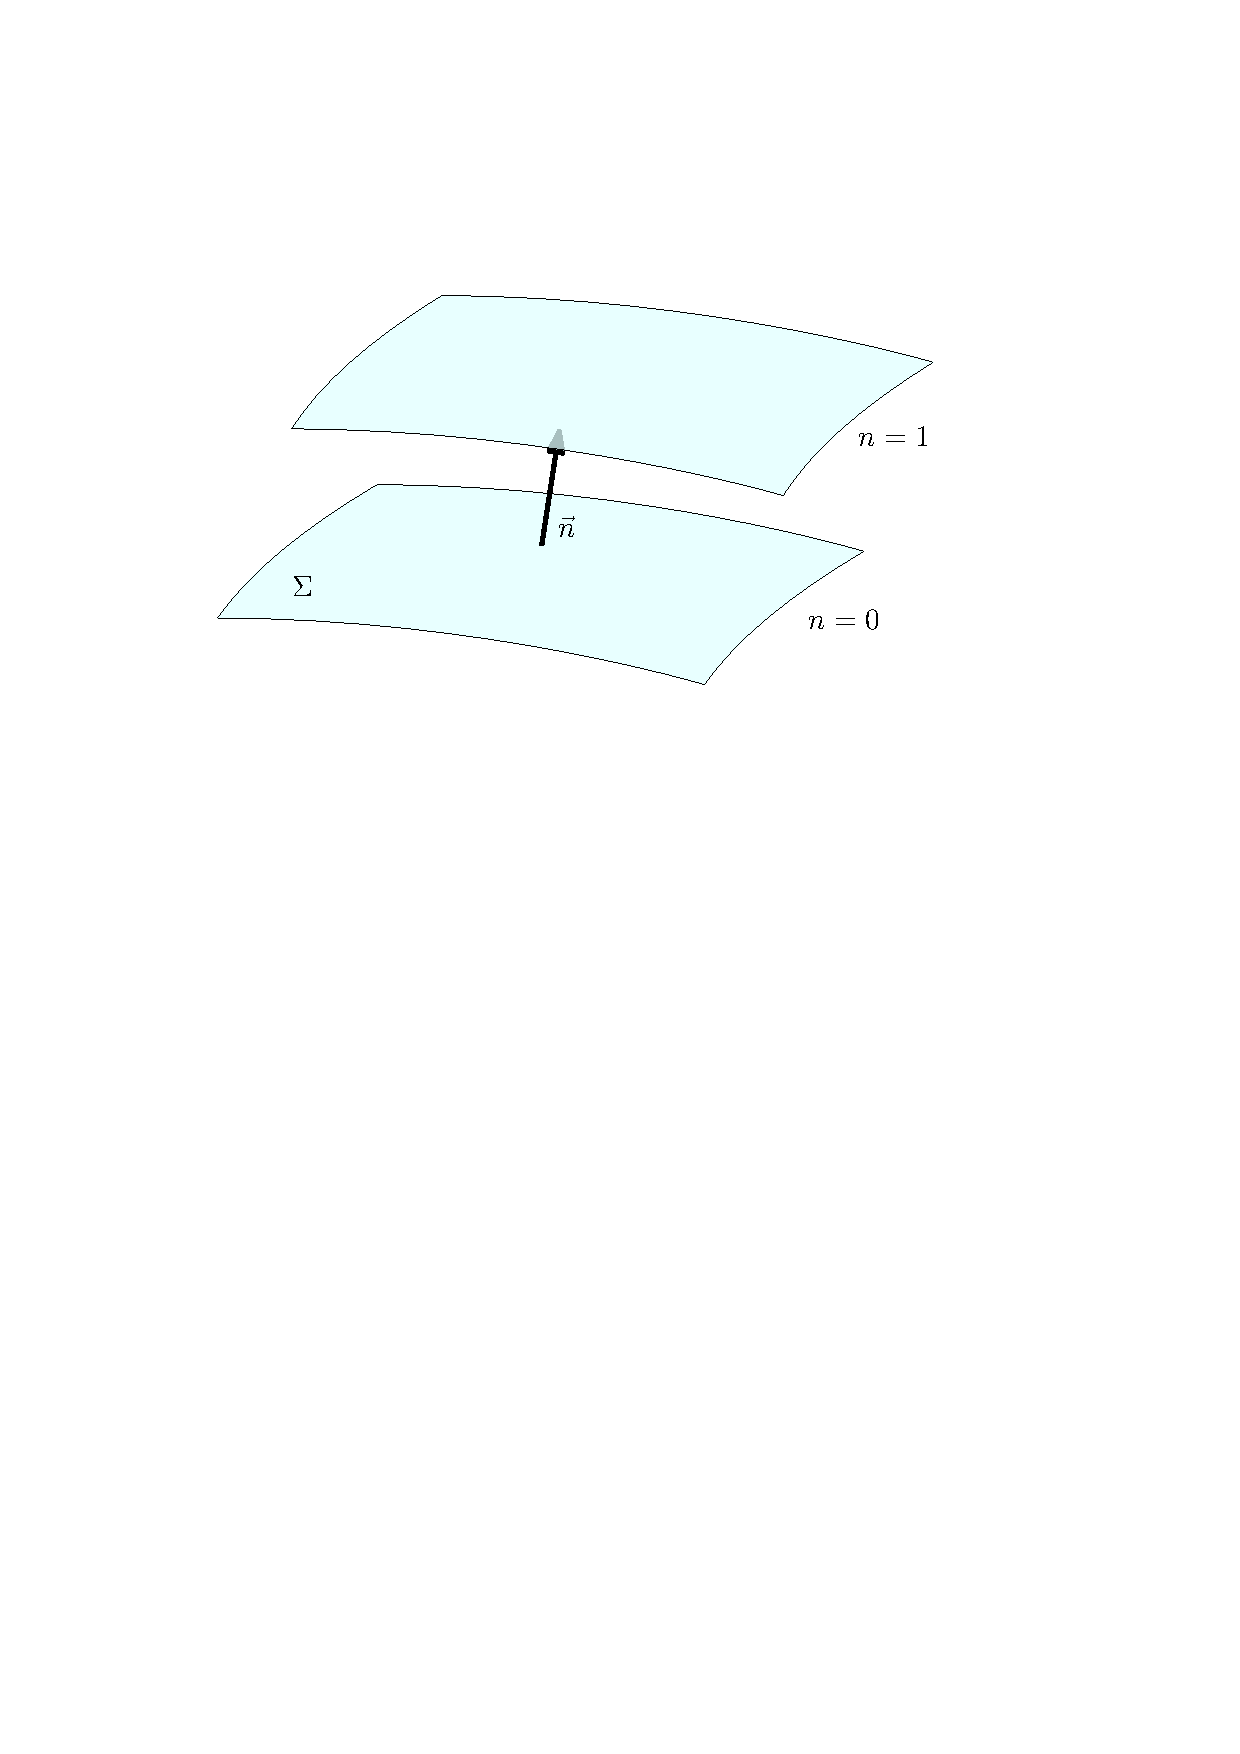
\includegraphics[width=0.7\linewidth]{figures/Junction.pdf}
     \caption{Coordenadas Gausianas en el vecindario a $\Sigma$}
     \label{JC}
 \end{figure}
Si a través de la superficie no hay contenido material, las condiciones de acoplamiento en estas coordenadas son:
 \begin{enumerate}[leftmargin=2cm]
     \item La métrica de las 3-superficies $g_{ij}$ es continua a través de $\Sigma$.
     \item El tensor de energía-momento superficial se anula
     \begin{equation}
\tensor{S}{^\alpha_\beta}\equiv\lim _{\varepsilon \rightarrow 0}\left[\int_{-e}^{+\varepsilon} T_{\beta}^{\alpha} d n\right]=0.
    \end{equation}
 \end{enumerate}

 Como es explicado en \cite{Misner1973} la condición 2 es equivalente a exigir la continuidad de la segunda forma fundamental. 
 
 \textbf{C2:} Para el caso considerado en este trabajo $\Sigma:\,r=R$, además la simetría esférica permite identificar $\vec{n}=\pdv{r}$ y debido a que la métrica exterior es la de Schwarzschild $\eval{T^{\alpha}_{\beta}}_{+\epsilon}$= 0, teniendo en cuenta estas consideraciones las condiciones de acoplamiento se reducen a
 \begin{enumerate}[leftmargin=2cm]
     \item $e ^ {  2 \nu(R) } =  1 - \frac { 2 M } { R }= e ^ { -2 \lambda(R) }$.
    \item $P(R)=\rho(R)=0$.
 \end{enumerate}


\subsection*{ Sobre el corrimiento al rojo gravitacional}
La luz emitida por una estrella es observada corrida al rojo por un observador lejano debido a la presencia del campo gravitacional. Qué tanto es corrida al rojo puede ser estimado de manera sencilla con u argumento basado en óptica geométrica \cite{Glendenning2000}: considerando un átomo de la estrella a una distancia $r$ de su centro, que emite un fotones con determinada frecuencia, el intervalo de tiempo propio entre dos emisiones consecutivas está dado por
\begin{equation}
d \tau=\sqrt{-g_{\mu \nu} d x^{\mu} d x^{\nu}},
\end{equation}
en el marco del átomo esto es simplemente ($dx^i=0$)
\begin{equation}
d \tau_{\mathrm{e}}=\sqrt{-g_{00}(r)} d t.
\end{equation}
El intervalo espacio-temporal para un rayo radial será
\begin{equation}
d \tau^{2}=g_{11}(r) d r^{2} - g_{00}(r) d t^{2} = 0,
\end{equation}
así que el tiempo que tardó un pulso en viajar de $r$ a $\infty$ es
\begin{equation}\label{timeinterval}
\Delta t=t_{\infty}-t_{r}= \int_{r}^{\infty}\left(\frac{g_{11}(\bar{r})}{g_{00}(\bar{r})}\right)^{1 / 2} d \bar{r}.
\end{equation}
Como $\Delta{t}$ no depende de $t$, el tiempo coordenado entre dos emisiones consecutivas $dt$, medido por un observador ubicado en $r$ es el mismo para el observador lejano. Con lo anterior en cuenta, el tiempo propio para el observador lejano será
\begin{equation}
d \tau_{\mathrm{o}}=\sqrt{-g_{00}(\infty)} d t.
\end{equation}
Como el inverso del tiempo propio es proporcional a la frecuencia, la razón entre la frecuencia emitida y observada es
\begin{equation}
\frac{\omega_{\mathrm{e}}}{\omega_{\mathrm{0}}}=\left(\frac{g_{00}(\infty)}{g_{00}(r)}\right)^{1 / 2}=e^{-\nu(r)},
\end{equation}
y con esto el corrimiento al rojo gravitacional es
\begin{equation}
    z(r)\equiv \frac{\omega_{\mathrm{e}}-\omega_{\mathrm{o}}}{\omega_{\mathrm{o}}}  = e^{-\nu(r)}-1.
    \label{redshift}
\end{equation}

\textbf{C3:} El corrimiento al rojo descrito por \eqref{redshift} debe disminuir con el incremento de $r$.
\subsection*{Sobre el signo de la densidad de energía y la presión}
Si bien la teoría cuántica de campos permite fenómenos de sub-vacío como la aparición de densidades de energía negativa locales \cite{Ford2010}, restricciones sobre magnitud y duración sugieren que es improbable que hayan consecuencias macroscópicas. Por esto se requiere que las densidades de energía sean positivas.
Así mismo, aunque los sistemas físicos pueden tener presiones negativas, esto solo ocurre en estados metaestables o de equilibrio parcial \cite{Landau1980}. Este tipo de estados tienen un determinado tiempo de relajación después del cual el sistema retorna a estados más estables. Por ende, como se estudiarán modelos estelares en equilibrio, se requiere la presión sea siempre positiva. 

\textbf{C4:} La densidad de energía y la presión deben ser positivas dentro de la estrella. 

\subsection*{Sobre la densidad de energía y la presión}
\textbf{C5:} La densidad de energía y la presión deben alcanzar un máximo en el centro ($\rho'(0)=P'(0)=0$) y deben decrecer monótonamente hacia afuera.

\subsection*{Condiciones de energía}
Con el fin de obtener soluciones a las ecuaciones de Einstein en presencia de fuentes de energía y momento realistas es necesario imponer ciertas condiciones de energía que limiten la arbitrariedad del tensor energía-momentum escogido.

Existe una variedad de condiciones de energía que son usadas en diferentes circunstancias, las usadas con mayor frecuencia son \cite{Hawking1973,Carroll2003}:

\begin{itemize}[leftmargin=1.5cm]
    \item \emph{Condición de energía débil (WEC)}: el tensor de energía-momentum en cada punto $p$ de la variedad obedece la desigualdad $T_{\mu \nu} t^{\mu} t^{\nu} \geq 0$ para cualquier vector tipo tiempo $t^{\mu}\in T_{p}$.
    \item \emph{Condición de energía dominante (DEC)}: el tensor de energía-momentum en cada punto $p$ de la variedad obedece la desigualdad $T_{\mu \nu} t^{\mu} t^{\nu} \geq 0$ y además $T^{\mu \nu} t_{\mu}$ es un vector que no es tipo espacio para cualquier vector tipo tiempo $t^{\mu}\in T_{p}$.
    \item \emph{Condición de energía fuerte (SEC)}: el tensor de energía-momentum en cada punto $p$ de la variedad obedece la desigualdad $T_{\mu \nu} t^{\mu} t^{\nu} \geq \frac{1}{2} T_{\lambda}^{\lambda} t^{\sigma} t_{\sigma}$, para cualquier vector tipo tiempo $t^{\mu}\in T_{p}$.
\end{itemize}
Mientras que las condiciones débil y fuerte no se cumplen para el tensor energía-momento de algunos campos escalares con $m=0$ y $m\neq 0$ respectivamente \cite{Hawking1973}, la dominante es cumplida por todas las formas de materia conocidas y se requerirá por lo tanto que la materia en las estrellas de neutrones la cumpla. La DEC incluye a la WEC, como se verá esta prohíbe que los observadores midan densidades de energía negativas. La condición extra obliga a que la energía y el momento locales fluyan de pasado a futuro.

Escribiendo $t^\nu$ en una tétrada ortonormal $e_{\mu}$ como
\begin{equation}
    t^{\mu} e_{\mu}= \left(1+a^{2}+b^{2}+c^{2}\right)^{1 / 2} e_{0}+a e_{1}+b e_{2}+c e_{3},
\end{equation}
con el tensor de energía-momento de un fluido perfecto que se está considerando \eqref{EMT}, la condición $T_{\mu \nu} t^{\mu} t^{\nu} \geq 0$ se puede escribir como
\begin{equation}
T_{\mu \nu} v^{\mu} v^{\nu}=\left(1+a^{2}+b^{2}+c^{2}\right) \rho + \left( a^{2} +b^{2} +c^{2} \right) P \geq 0 \quad \forall a,b,c \in \mathbb{R},
\end{equation}
para el caso $a=b=c=0$ esto implica $\rho \geq 0$ y en el límite en que $a^2+b^2+c^2 \to \infty$ que $\rho + P \geq 0$.

Además, con $T^{\mu \nu} t_{\mu}$ escrito como
\begin{equation}
T^{\mu \nu} t_{\mu}e_{\nu}=\left(1+a^{2}+b^{2}+c^{2}\right)^{1 / 2} \rho e_{0}+a P e_{1}+b P e_{2}+c P e_{3},
\end{equation}
la condición de que no sea tipo espacio se convierte en
\begin{equation}
    -\rho^2 + (P^2-\rho^2)(a^2+b^2+c^2) \leq 0 \quad \forall a,b,c \in \mathbb{R},
\end{equation}
lo cual implica que $\rho \geq |P|$.

Debido a que en C1 se requirió que $\rho$ y $P$ fueran positivas, la condición de energía dominante añade la restricción $\rho \geq P$.

\textbf{C6:} La solución debe satisfacer la condición $\rho \geq P$.

\subsection*{Condición de causalidad}
El postulado de causalidad local en relatividad general prohíbe que una señal se propague a una velocidad mayor que la velocidad de la luz \cite{Hawking1973}. 

\textbf{C7:}  La velocidad del sonido en la estrella (modelada como un fluido perfecto) está dada por 
\begin{equation}
    v^2=\dv{P}{\rho},
\end{equation}
y esta no puede sobrepasar la velocidad de la luz:
\begin{equation}
    0 < \dv{P}{\rho} \leq 1 .
\end{equation}

\subsection*{Estabilidad ante pulsaciones radiales}

La teoría de oscilaciones radiales infinitesimales fue desarrollada por Chandrasekhar \cite{Chandrasekhar1964a}. En este enfoque se introduce un desplazamiento Lagrangiano (medido por un observador que se mueve con el fluido) $\xi(r,t)$ y se estudia su evolución dinámica de acuerdo a las ecuaciones de Einstein, la conservación local de la energía-momento y las leyes de la termodinámica, todas propiamente linealizadas.

Se puede demostrar \cite{Chandrasekhar1964a,Misner1973} que al suponer un desplazamiento con una dependencia temporal sinusoidal $\xi(r, t)=\mathrm{e}^{-\mathrm{i} \omega t} \zeta(r)$  y condiciones de frontera apropiadas, la ecuación que gobierna la dinámica de las perturbaciones radiales se convierte en un problema de autovalores para la frecuencia del desplazamiento $\omega$. La condición de estabilidad en este esquema se reduce al requerimiento $\omega \geq 0$, ya que para $\omega<0$ el desplazamiento $\xi(r,t)$ crece exponencialmente con el tiempo.   

Los diferentes criterios de estabilidad ante pulsaciones radiales se diferencian en la función de prueba $\zeta$ escogida y las aproximaciones que se hagan para obtener condiciones simples que aseguren $\omega \geq 0$.


\subsection*{Criterio de estabilidad del índice adiabático }

Chandrasekhar aplicó el formalismo para mostrar que las condiciones suficientes para la estabilidad dinámica (de distribuciones esféricas de materia) son más restrictivas en relatividad general que en la teoría Newtoniana. Como ejemplo, se puede comparar el límite inferior Newtoniano para el índice adiabático, necesario para asegurar la  estabilidad
\begin{equation}
    \gamma \equiv \frac { \rho + P  } { P } \dv{P}{\rho} \geq \frac{4}{3},
\end{equation}
con lo obtenido en relatividad general para una esfera de densidad e índice adiabático constantes
\begin{equation}
    \gamma \geq \frac{4}{3}  \frac{19}{42} \frac{2M}{R}.
\end{equation}

Una condición más realista para asegurar la estabilidad, la cual toma en cuenta que el índice adiabático depende de la coordenada $r$, fue formulada por Merafina y Ruffini \cite{Merafina1989} en términos de un índice adiabático efectivo $\langle\gamma\rangle$ definido como

A\begin{equation}
    \langle\gamma\rangle\equiv\frac{\int_{0}^{R} e^{\lambda+3 \nu} \gamma(r) P(r) r^{2} d r}{\int_{0}^{R} e^{\lambda+3 \nu} P(r) r^{2} d r}.
\end{equation}

\textbf{C8:} El índice adiabático efectivo debe satisfacer
\begin{equation}
     \langle\gamma\rangle \geq \gamma_{cr},
\end{equation}
donde $\gamma_{cr}$ está dado por
\begin{align}
    \gamma_{cr} = \frac{4}{3} +& \frac{1}{36} \frac{\int_{0}^{R} e^{\lambda+3 \mathrm{v}}\left[16 P+\left(e^{\lambda}-1\right)\left(P+\rho \right)\right]\left(e^{\lambda}-1\right) r^{2} d r}{\int_{0}^{R} e^{\lambda+3 \mathrm{v}} P r^{2} d r} \nonumber
    \\ &+ \frac{4 \pi}{9} \frac{\int_{0}^{R} e^{3( \lambda+ \mathrm{v})}\left[8 P+\left(e^{\lambda}+1\right)\left(P+\rho \right)\right] P r^{4} d r}{\int_{0}^{R} e^{\lambda+3 \mathrm{v}} P r^{2} d r}
    \\ & + \frac{16 \pi^{2} }{9} \frac{\int_{0}^{R} e^{5 \lambda+3 v }\left(P+\rho \right) P^{2} r^{6} d r}{\int_{0}^{R} e^{\lambda+3 v } P r^{2} d r}. \nonumber
\end{align}

\subsection*{Criterio de Harrison-Zeldovich-Novikov}

La condición C8 es una condición suficiente para la estabilidad ante pulsaciones radiales. Zel'dovich \& Novikov \cite{Zeldovich1971} y Harrison, et al. \cite{Harrison1965} formularon una condición de estabilidad necesaria que es más fácil de aplicar. Usando diferentes argumentos, identificaron que para un modo normal y EOS dados, la frecuencia de las pulsaciones $\omega$ pasa de ser positiva a negativa en el mismo valor de la densidad central $\rho_c$ para el cual se alcanza la masa máxima $M_{\text{max}}$. 

Así que una manera sencilla de identificar modelos que sean inestables es usar el diagrama $M(\rho_c)$ para identificar el valor de $\rho_c$ para el cual se alcanza el máximo, los modelos con $\rho_c$ mayor serán inestables. 

\textbf{C10:} Para una configuración sea estable respecto a oscilaciones radiales es \emph{necesario} que su masa $M$ aumente a medida que la densidad central $\rho_{c}$ crece: 

\begin{equation}
    \frac { \partial M \left( \rho _ { c } \right) } { \partial \rho _ { c } } > 0.
\end{equation}
Además, los puntos en los que $\frac { \partial M \left( \rho _ { c } \right) } { \partial \rho _ { c } } = 0$ (puntos críticos) son puntos donde la configuración pasa de estabilidad a inestabilidad.



\subsection*{Estabilidad ante cracking}
\noindent El cracking es una posible inestabilidad de esferas anisótropas ($P_r \neq P_{\perp}$) ante perturbaciones locales de densidad. Cuando estas perturbaciones son constantes, se puede demostrar \cite{Abreu2007} que las configuraciones estables ante cracking deben satisfacer
\begin{equation}\label{abreucracking}
    -1 \leq v_{s \perp}^{2}-v_{s r}^{2} \leq 0.
\end{equation}
Además, como fue demostrado por \cite{Ivanov2017} \eqref{abreucking} es equivalente al requerimiento
\begin{equation}
    0 \geq \frac{\mathrm{d} P_{\perp}}{\mathrm{d} r} \geq \frac{\mathrm{d} P}{\mathrm{d} r}.
\end{equation}
Para modelos isótropos ($P_r=P_{\perp}=P$), esto se reduce a 
\begin{equation}
    0 \geq \frac{\mathrm{d} P}{\mathrm{d} r},
\end{equation}
esta condición asegura que la presión decrece monótonamente y por lo tanto concuerda con la condición C5.

\textbf{C9:} El criterio para que una distribución sea estable ante cracking, en el caso de perturbaciones de densidad constantes, es 
\begin{equation}
    \dv{P}{r} \leq 0.
\end{equation}


\subsection*{Estabilidad ante convección adiabática}

La estabilidad contra convección se puede entender como sigue: cuando un elemento de fluido es desplazado rápidamente hacia abajo, si su densidad aumenta más rápido que la densidad que lo rodea, el elemento se hundirá y la configuración será inestable. Por otro lado, si la densidad del elemento de fluido es menor que la de su alrededor, este flotará y la estrella será estable ante convección \cite{Bondi1964a}. 

Hernández et al. derivaron en \cite{Hernandez2018} una condición sencilla que asegura estabilidad ante la convección adiabática. Siguiendo su trabajo: si se denota a $\rho(r_p)$ como la densidad de un elemento de fluido en su posición original $r_p$ y se desplaza el elemento hacia abajo, se tiene
\begin{equation}
    \rho\left(r_{p}\right) \rightarrow \rho\left(r_{p}\right)+\delta \rho(r),\quad \text {con } \quad \delta \rho(r)=\rho^{\prime}(r)(-\delta r) \quad \text { y } \quad r=r_{p}-\delta r,
\end{equation}
donde $r$ es la nueva posición del elemento de fluido y $-\delta r$ el desplazamiento hacia el centro. 
Como $\rho^{\prime} < 0$, $\delta \rho(r)$ es positivo y la densidad del elemento de fluido que fue comprimido será mayor en $r$ que en $r_p$. 
Expandiendo la densidad del ambiente en $r$ a primer orden en $-\delta r$ se obtiene
\begin{equation}
    \rho\left(r_{p}-\delta r\right) \approx \rho\left(r_{p}\right)+\rho^{\prime}\left(r_{p}\right)(-\delta r).
\end{equation}
Según lo ya explicado, el sistema será estable si la densidad del ambiente es mayor o igual a la densidad del elemento de fluido:
\begin{align*}
    \rho\left(r_{p}\right)+\rho^{\prime}\left(r_{p}\right)(-\delta r) &\geq \rho\left(r_{p}\right)+\rho^{\prime}(r)(-\delta r) \\ \rho^{\prime}\left(r_{p}\right) &\leq \rho^{\prime}(r).
\end{align*}
Expandiendo ahora $\rho^{\prime}(r)$ alrededor $r_p$ se obtiene
\begin{equation}
    \rho^{\prime}\left(r_{p}\right)+\rho^{\prime \prime}\left(r_{p}\right) \delta r \leq \rho^{\prime}\left(r_{p}\right),
\end{equation}
de donde se obtiene el criterio de estabilidad ante convección adiabática
\begin{equation}
    \rho^{\prime \prime}(r) \leq 0.
\end{equation}

En principio parece que este criterio es válido solo para perturbaciones muy rápidas: así asegura que la escala de tiempo hidrodinámica $\tau_h$ sea menor a la escala de tiempo térmica $\tau_t$ y se puede ignorar el transporte de calor. Sin embargo, es sabido que $\tau_h \ll \tau_t$ durante todas las fases de evolución estelar \cite{Bisnovatyi-Kogan2011}, por lo que el criterio es válido en situaciones más generales.  

\textbf{C11:} Para que un modelo estelar sea estable ante movimientos convectivos adiabáticos, el perfil de densidad $\rho(r)$ debe cumplir: 
\begin{equation}
    \rho ^ { \prime \prime } ( r ) \leq 0.
\end{equation}